\section{需求}
\subsection{功能需求}
\label{c31}
%地面站系统包括串口通信,飞控连接,飞行参数显示与记录,地图显示,任务航线规划,无人机指令,飞控更新和地面站设置等功能。
\subsubsection{串口通信}
地面站系统使用串口通过直接连接或经由数传电台与无人机飞控进行通信。
串口通信波特率为115200,可以通过地面站设置更改串口使用的波特率。

串口通信根据通信协议解析接收缓存并提取数据包,供其他功能模块使用,或接受其他功能模块传递的数据包,将其转换为数据流经由串口发送。

当串口意外断开时,软件能够捕获异常并做适当处理,保证运行的稳定。

\subsubsection{飞控连接}
地面站软件只会同时与一台无人机建立连接。

当连接正常接入时,软件能够自动识别连接使用的串口,接入的硬件和使用的通讯协议,并在10s内与飞控建立连接。
连接建立后忽略所有新出现的串口连接。软件通过检测心跳包判断连接是否可用,当一定时间没有接收到心跳包后认为连接断开。心跳包丢失时间可在软件中进行设置。

在建立连接前,若存在无法识别通信协议的串口连接,软件将使用串口通信设置的波特率持续对串口进行扫描,直到出现可识别的串口。

\subsubsection{飞行参数显示与记录}
地面站系统建立连接后与无人机飞控进行通信,解析数据包获取飞行数据,并以一定的方式将其中的部分参数显示在软件界面中。界面中直接显示的数据见表\ref{t3dppara}。
对于接收到的数据,软件以与飞控机载日志相同的格式进行记录,并将记录保存在硬盘中。
所有数值全部使用SI单位。

对于不同的飞控硬件,发回的数据内容可能并不相同。若飞控没有发送需要显示的参数,地面站中将显示参数的缺省值。
若飞控中途断开连接,软件将保持显示最后一次接收到的数值。

\begin{table}[ht]
\centering
\caption{显示的飞行参数}
\label{t3dppara}
\begin{tabular}{|l|l|}
\hline
\multicolumn{1}{|c|}{参数类型} & \multicolumn{1}{c|}{参数名}  \\ \hline
飞行姿态 & 俯仰角,滚转角,机头指向              \\ \hline
飞行状态 & 空速,地速,航向,上升/下降率,相对高度,飞行模式 \\ \hline
定位状态 & 精度,纬度,卫星数,定位状态,定位误差       \\ \hline
导航状态 & 航程,航时,回航角,航点信息            \\ \hline
动力状态 & 电池电压,电池电流,估计剩余电量          \\ \hline
通信状态 & 通信速率,通信协议,RSSI            \\ \hline
\end{tabular}
\end{table}

\subsubsection{地图显示}
地面站系统能够显示普通地图,卫星地图或混合地图,并能够在三种地图之间切换。地图显示部分占据地面站界面的主要部分,能够自由进行移动和缩放。
除地图外,还能够在地图上实时显示无人机位置,方向,飞行轨迹和预设航线。

地图使用国内电子地图平台,地图上显示误差不超过0.1m。

\subsubsection{任务航线规划}
地面站系统能够进行任务航线规划,任务由一系列按顺序相连的任务项组成。使用的任务项如表\ref{t3miss}所示。
任务项通过点击地图或输入参数设置,或通过子任务加载或自动生成。任务航线可以保存到本地文件,或从文件中读取。

任务规划完毕后通过串口通信发送至无人机飞控,飞控不支持的任务项类型将被自动忽略。

\begin{table}[ht]
\centering
\caption{任务项}
\label{t3miss}
\begin{tabular}{|l|l|}
\hline
\multicolumn{1}{|c|}{类别} & \multicolumn{1}{c|}{任务项} \\ \hline
航路点                      & 初始点,导航点,起降点,环绕点          \\ \hline
动作                       & 拍照,投放载荷,模态转换,操作任务载荷      \\ \hline
子任务                       & 子任务,扫描区域                 \\ \hline
飞行控制                     & 改变速度,改变高度                \\ \hline
\end{tabular}
\end{table}

\subsubsection{无人机指令}
地面站系统能够直接向无人机飞控发送指令,指示飞控完成一定的动作。发送的指令主要包括以下几类:
\begin{itemize}
\setlength{\itemsep}{-2pt}
\item 飞行指令:控制无人机飞行的指令,包括起飞,降落,返航,飞行模式切换,飞行到目标点等。
\item 飞控指令:命令飞控执行动作,包括校准传感器,锁定或解锁飞控,获取和设置飞控参数等。
\item 任务指令:与任务相关的指令,包括发送和接收任务或单独的任务项,开始或终止任务等。
\end{itemize}

指令发送后由地面站判定是否发送成功,若发送失败将自动重发若干次,重发次数可由用户设定。

\subsubsection{双显示器显示}
地面站系统能够拆分为两个窗口,分别显示于两个显示器中。
其中一个窗口显示地图和飞行参数,另一个窗口显示机载摄像设备传回的画面。
在运行过程中两个窗口可以快速交换。

若无视频流传入,则摄像画面窗口显示空白内容。

\subsubsection{视频图像显示与记录}
地面站系统能够显示无人机传回的画面。无人机经图传电台将画面传回地面站。
地面站系统通过视频采集卡获取视频流,将视频画面显示在视频界面中,同时将视频实时保存至硬盘。

地面站系统显示视频画面时可以在画面上叠加部分飞行参数和图形提示,以便操作手快速获取信息。

\subsubsection{飞行日志读取和回放}
地面站系统能够读取飞行日志和视频记录,并进行回放。
回放时可以单独回放飞行参数和轨迹,或同时回放飞行参数和视频画面。
回放速度和进度均可以手动实时调节。

\subsubsection{飞控更新}
地面站系统能够对飞控固件进行更新和刷写。

\subsubsection{地面站设置}
对地面站软件中的参数进行设置。

\subsection{外部接口需求}

\subsubsection{接口标识和接口图}
地面站系统外部接口如图\ref{f3int}所示。
\begin{figure}[ht]
	\begin{center}
		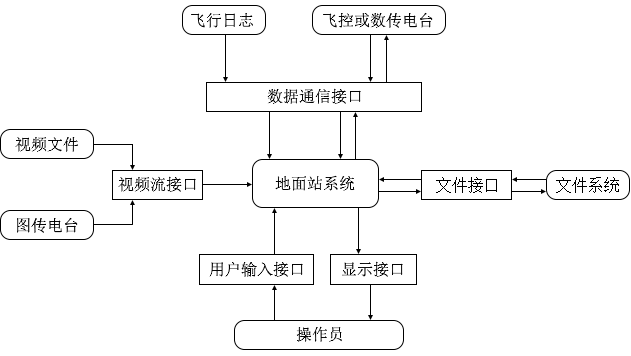
\includegraphics{interface.png}
		\caption{外部接口图}
		\label{f3int}
	\end{center}
\end{figure}

\subsubsection{飞控通信接口}
至少支持MAVLINK 1.0 通信协议,见引用文档MAVLink Micro Air Vehicle Communication Protocol。


\subsection{计算机资源需求}
\subsubsection{计算机硬件需求}
运行地面站软件的计算机硬件需求配置如表\ref{t3req}所示。
\begin{table}[ht]
\centering
\caption{计算机硬件需求}
\label{t3req}
\begin{tabular}{|l|l|}
\hline
\multicolumn{1}{|c|}{硬件} & \multicolumn{1}{c|}{最低需求} \\ \hline
处理器                      & Intel Core i5             \\ \hline
内存                       & 4G                        \\ \hline
图形                       & Intel HD530               \\ \hline
储存空间                     & 1G SSD                    \\ \hline
显示                       & 每个显示器实际分辨率1366*768        \\ \hline
\multirow{2}{*}{其他}      & 至少一个USB接口                 \\ \cline{2-2} 
                         & 支持DirectShow的视频采集卡        \\ \hline
\end{tabular}
\end{table}


\subsubsection{计算机软件需求}
地面站系统需要在安装有Windows 7及以上的Windows操作系统运行。
系统必须包含Microsoft .NET Framework 4.5和4.0运行库,
必须包含DirectX 9.0c及以上运行库。
需包含与飞控或数传电台连接的串口驱动程序。
需包含视频采集相关驱动程序。
\endinput